\documentclass[11pt]{article}
\usepackage[utf8]{inputenc}
\usepackage{amstext}
\usepackage{amsmath}
\usepackage{graphicx}
\usepackage{textcomp}
\usepackage{float}
\usepackage{varioref}
%\usepackage{fancyref}
\usepackage{caption}
\usepackage{subcaption}
%\usepackage{comment}
\usepackage{hyperref}
\usepackage{epstopdf}
\usepackage{ esint }
\usepackage{wrapfig}
\usepackage[margin=1in, paperwidth=8.5in, paperheight=11in]{geometry}

\title{Computer Networks Datalink Standard RFC}
\author{Computer Networks, Olin College\textsuperscript{1}}
%\date{February 2014}

\begin{document}

\footnotetext[1]{Document compiled by Dakota Nelson. Standards committee composed of Ezra Varady, Dakota Nelson, Ian Hill, Ben Tang, Ryan Louie, and Jennifer Wei.}

\maketitle

\section{Introduction}

In order to enable the transmission of multiple protocols across a common bus, the following standard has been proposed. Adherence to this standard will allow relatively efficient transmission, with collision detection and error correction, of multiple incompatible packet types, with varying transmission speeds, across a single bus.

For the purposes of this document, a node which is attempting to transmit a message is designated the `sender,' the node this message is directed to is designated the `reciever,' all other nodes listening for the same protocol will be designated as `similar nodes,' and all other nodes listening for different protocols will be designated `foreign nodes.'

The common communication method being shared between nodes will be known as the `bus.' In this document, the bus is assumed to be effectively a single wire, with no external clock.

Baud rate\textsuperscript{2} is defined as the number of pulses per second. For example: one Morse code `dot' at one baud equates to bringing the bus high for one second, whereas a `dash' would be three seconds. At two baud, the `dot' would be a half second, the `dash' would be 1.5 seconds, and so on.

\footnotetext[2]{See: \url{https://en.wikipedia.org/wiki/Baud}}

\section{The Multi-Protocol Data Link Layer Standard}

In essence, the protocol is as follows:

\begin{figure}[!ht]
\centering
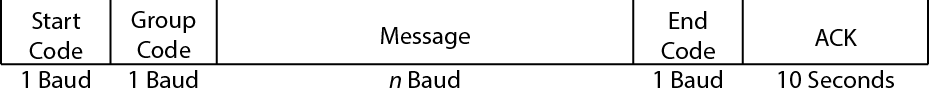
\includegraphics[width=\textwidth]{datalink_diagram.png}
\caption{A pictoral representation of the standard.}
\label{fig:standard}
\end{figure}

\subsection{Start Code}

In order to signal that a message is about to begin, the sender will transmit a 'high' signal for 4 seconds. In conjunction with the collision avoidance protocol (see Section \ref{sec:collision_avoidance}), this serves to clear the bus.

\subsection{Group Code}

After the start code has been transmitted, the sender has taken ownership of the bus. At this point, the sender pulls the bus low for one second in order to signal the end of the start signal, then transmits a group code, at a rate of one baud. This group code uniquely identifies the protocol which will follow. This group code is composed of a single base-36 number, thus allowing it to be transmitted as one Morse code character.

\subsection{Message}

After the group code has been transmitted, the sender transmits a message, at any baud rate, using whatever protocol it wishes, with two exceptions:
\begin{description}
\item[First]\hspace{-6pt}, the message may not contain the Morse code prosign `+'\textsuperscript{3}.
\item[Second]\hspace{-6pt}, the message may not bring the bus high for longer than 3 seconds.
\end{description}

Since this message has been uniquely identified using the group code, only similar nodes need recieve it, while all foreign nodes may simply ignore the message and wait for the protocol's end code.

\begin{wrapfigure}{R}{0.25\textwidth}
\vspace{-40pt}
\centering
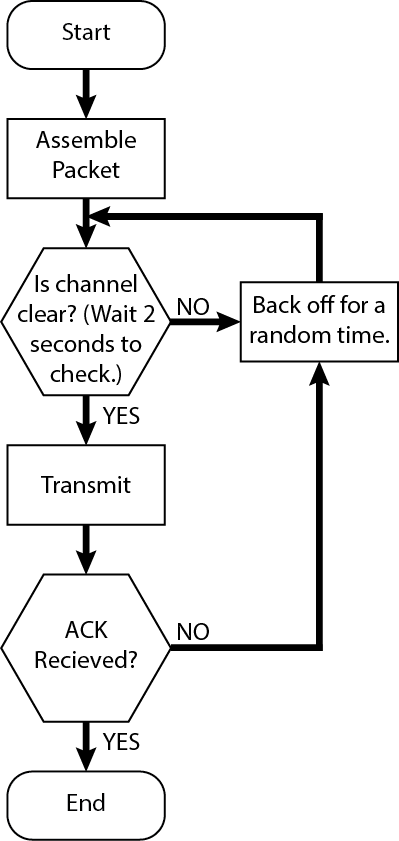
\includegraphics[width=.3\textwidth]{CSMA_Flow.png}
\caption{The collision avoidance algorithm.}
\label{fig:CSMA}
\end{wrapfigure}

\footnotetext[3]{See: \url{https://en.wikipedia.org/wiki/Prosigns_for_Morse_code}}

\subsection{End Code}

Once the sender has finished transmitting its message, the end code must be transmitted to signal that the message has concluded and to relinquish control of the bus. This end code is the morse code prosign `+'\textsuperscript{3}, transmitted at a rate of one baud.

\subsection{ACK}


Once the sender has transmitted the end code, all nodes on the network must not transmit for 10 seconds. This space is to allow the reciever to transmit an ACK message to inform the sender that the message was successfully recieved.

This ACK message is simply the group code of the reciever (and thus also of the sender). If the sender recieves an ACK matching the group code of its transmission, the message is assumed good, else the message must be retransmitted.

\section{Collision Avoidance}
\label{sec:collision_avoidance}

In order that collisions should be avoided, any node which detects a transmission while it is transmitting or intending to transmit will immediately abort that transmission and back off for $n$ seconds, where $n$ is a random time selected from a Gaussian distribution centered around 20 seconds. Before transmitting, a node must listen to the bus for at least two seconds before attempting to transmit the start code. A diagram of this process is shown in Figure \ref{fig:CSMA}.

\end{document}
